\mysubsectionformatted{Design Pattern Proxy}
\myparagraph{

\begin{tcolorbox}[colback=blue!5!white, colframe=blue!75!black]
    Il pattern permette l'accesso a quegli oggetti che non sono direttamente\\ accessibili
    o non si desidera fornire l'accesso diretto. Viene creato un oggetto proxy che implementa
    la stessa interfaccia dell'oggetto ed è responsabile del controllo o del miglioramento dell'accesso
    a questo oggetto.
\end{tcolorbox}
\vspace{0.1cm}
    
\begin{center}
    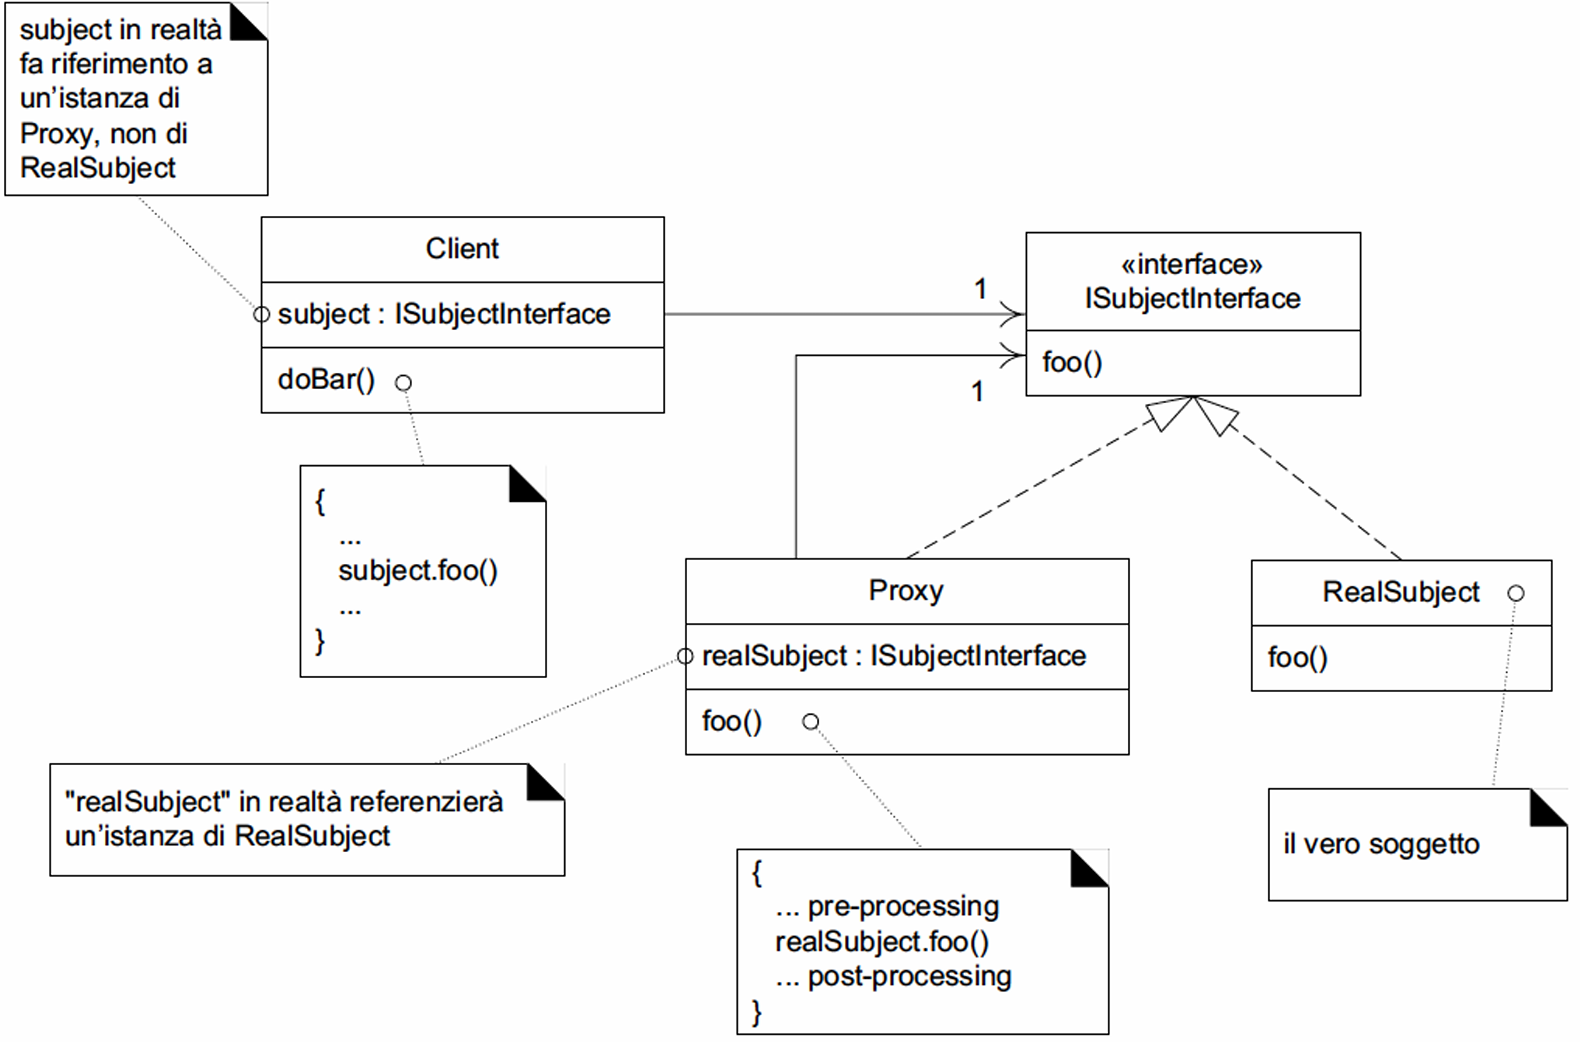
\includegraphics[scale=0.25]{Esercitazione - Design Patterns/proxy_pattern.png}
\end{center}
I componenti del pattern sono:
\begin{enumerate}
    \item \textbf{SubjectInterface} definisce un'interfaccia comune per l'oggetto reale\\ \textbf{RealSubject}
    e il \textbf{Proxy}, permettendo di usarli in modo alternabile.
    \item \textbf{RealSubject} è l'oggetto reale, contiene l'implementazione concreta della logica principale.
    \item \textbf{Proxy} è la classe che implementa la \textbf{SubjectInterface} e controlla l'accesso all'oggetto
    reale, implementando logica extra, contiene un riferimento al \textbf{RealSubject}.
\end{enumerate}
Esistono due strategie di gestione della cache:
\begin{enumerate}
    \item \textbf{Inizializzazione lazy}: la cache viene riempita lentamente man mano che vengono inseriti gli oggetti.
    \item \textbf{Inizializzazione greedy}: la cache viene caricata all'inizio.
\end{enumerate}

\newpage

\mysubsubsectionformatted{Ultime considerazioni sul Proxy}
\begin{enumerate}
    \item Il Proxy è un oggetto esterno che nasconde un oggetto interno.
    \item Il client non sa che sta facendo riferimento al Proxy, ma crede di comunicare direttamente con il sistema interno.
    \item Il Proxy è utile nel caso sia necessaria una ridirezione dei messaggi. 
\end{enumerate}

\newpage
    
}